\section{Results}
This section will include details about all the results gathered throughout this experiment in a table format.ThiS allowing for comparisons between the different variations of Compling a C program.

\subsection{Figures}
Include good quality graphs.  These were produced by the Octave code presented in listings~\ref{lst:FormatFig} and~\ref{lst:PlotExample}.  You can play around with the \texttt{PaperSize} and \texttt{PaperPosition} variables to change the aspect ratio.  An easy way to obtain more space on a paper is to use wide, flat figures, such as Fig.

\begin{figure}[htd]
 \centering
 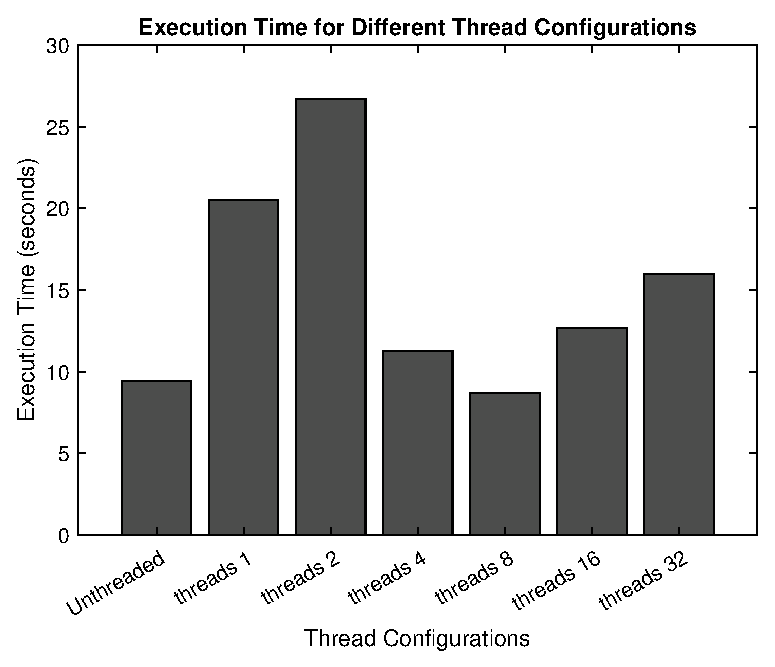
\includegraphics[width=0.5\textwidth]{bargraf_on_C_Threaded}
 \caption{Bar graph representing different C threading configurations.}
 \label{fig:threading}
\end{figure}

\begin{Matlab_float}{Octave function to format a figure and save it to a high quality PDF graph}{FormatFig}
function FormatFig(X, Y, File);
 set(gcf, 'PaperUnits'      , 'inches');
 set(gcf, 'PaperOrientation', 'landscape');
 set(gcf, 'PaperSize'       ,       [8, 4]);
 set(gcf, 'PaperPosition'   , [0, 0, 8, 4]);

 set(gca, 'FontName', 'Times New Roman');
 set(gca, 'Position', [0.1 0.2 0.85 0.75]);

 xlabel(["\n" X]);
 ylabel([Y "\n\n"]);

 setenv("GSC", "GSC"); # Eliminates stupid warning
 print(...
  [File '.pdf'],...
  '-dpdf'...
 );
end
\end{Matlab_float}

\begin{Matlab_float}{Example of how to use the FormatFig function}{PlotExample}
figure;                                   # Create a new figure
# Some code to calculate the various variables to plot...
plot(N, r, 'k', 'linewidth', 4); grid on; # Plot the data
xlim([0 360]);                            # Limit the x range
ylim([-1 1]);                             # Limit the y range
set(gca, 'xtick', [0 90 180 270 360]);    # Set the x labels

FormatFig(...                             # Call the function with:
 'Phase shift [\circ]',...                      # The x title
 'Correlation coefficient',...                  # The y title
 ['r_vs_N;_f=' num2str(f) ';_P=' num2str(P)]... # Format the file name
);
close all;                                # Close all open figures
\end{Matlab_float}

Always remember to include axes text, units and a meaningful caption in your graphs.  When typing units, a \micro{} sign has a tail!  The letter ``u'' is not a valid unit prefix.  When typing resistor values, use the \Ohm{} symbol.

\subsection{Tables}


\Table{Benchmarking and Non-threaded tests and Times (ms)}{ccc}{
 & \textbf{Python} & \textbf{C} \\
 \textbf{Test} & Golden Measure & Non-threaded
}{
 \textbf{1} & 403 & 11,1 \\
 \textbf{2} & 412 & 15,1 \\
 \textbf{3} & 406 & 6,12 \\
 \textbf{4} & 367 & 7,07 \\
 \textbf{5} & 383 & 7,65 \\
 \hline
\textbf{Average} & 394 & 9,41 \\
}{Test1}

\Table{Threaded tests and Times (ms)}{ccccccc}{
 \multicolumn{1}{c}{} & \multicolumn{6}{c}{\textbf{Threads}} \\
 \textbf{Test} & 1 & 2 & 4 & 8 & 16 & 32
}{
 \textbf{1} & 11,2 & 1,59 & 17,3 & 8,36 & 1,46 & 3,40 \\
 \textbf{2} & 10,5 & 11,2 & 6,71 & 11,3 & 8,90 & 4,88 \\
 \textbf{3} & 25,5 & 31,2 & 22,1 & 10,9 & 26,0 & 24,4 \\
 \textbf{4} & 40,4 & 37,5 & 2,59 & 11,3 & 2,07 & 17,8 \\
 \textbf{5} & 14,9 & 52,0 & 7,66 & 1,65 & 24,8 & 29,5 \\
 \hline
 \textbf{Average} & 20,5 & 26,7 & 11,3 & 8,70 & 12,6 & 16,0 \\
}{Test2}

\Table{Compiler Optimisation Flags tests and Times (ms)}{cccccccc}{
 \multicolumn{1}{c}{} & \multicolumn{7}{c}{\textbf{Optimisation Flags}} \\
 \textbf{Test} & -O0 & -O1 & -O2 & -O3 & -Ofast & -Os & -Og
}{
 \textbf{1} & 30,4 & 14,1 & 28,2 & 28,7 & 7,10 & 21,0 & 32,8 \\
 \textbf{2} & 34,7 & 33,3 & 20,9 & 26,9 & 12,3 & 5,78 & 8,92 \\
 \textbf{3} & 8,45 & 8,09 & 36,6 & 6,02 & 19,0 & 5,03 & 21,8 \\
 \textbf{4} & 12,1 & 6,19 & 5,31 & 9,71 & 5,87 & 24,2 & 6,22 \\
 \textbf{5} & 35,1 & 48,4 & 7,77 & 53,4 & 29,1 & 5,73 & 25,3 \\
 \hline
 \textbf{Average} & 24,2 & 22,0 & 19,8 & 24,9 & 14,7 & 12,3 & 19,0 \\
}{Test3}

\Table{COFs with \textit{-funroll-loops} tests and Times (ms)}{ccccc}{
 \multicolumn{1}{c}{} & \multicolumn{4}{c}{\textbf{Optimisation Flags}} \\
 \textbf{Test} & -O0 & -O3 & -Ofast & -Os
}{
 \textbf{1} & 43,9 & 7,31 & 24,6 & 6,01 \\
 \textbf{2} & 6,18 & 6,78 & 5,08 & 5,67 \\
 \textbf{3} & 12,1 & 15,1 & 42,7 & 11,8 \\
 \textbf{4} & 31,7 & 57,9 & 6,06 & 21,1 \\
 \textbf{5} & 13,4 & 34,0 & 6,21 & 5,47 \\
 \hline
 \textbf{Average} & 21,5 & 24,2 & 16,9 & 10,0 \\
}{Test4}

\Table{C Bit Widths tests and Times (ms)}{cccc}{
 \multicolumn{1}{c}{} & \multicolumn{3}{c}{\textbf{Data type}} \\
 \textbf{Test} & double & float & \textunderscore \textunderscore fp16
}{
 \textbf{1} & 31,9 & 6,69 & 110 \\
 \textbf{2} & 39,2 & 31,1 & 101 \\
 \textbf{3} & 34,1 & 10,9 & 26,2 \\
 \textbf{4} & 69 & 35 & 98,8 \\
 \textbf{5} & 12,1 & 7,87 & 93,8 \\
 \hline
 \textbf{Bit widths} & 64 & 32 & 16 \\
 \textbf{Average} & 37,26 & 18,312 & 85,96 \\
}{Test5}

\Table{Fastest Test}{cc|cc}{
 \textbf{Section} & \textbf{Fastest} & \textbf{Test} & \textbf{Time (ms)}
}{
 \textbf{Language} & C & \textbf{1} & 14,3 \\
 \textbf{Threaded} & True & \textbf{2} & 1,68 \\
 \textbf{Threads} & 8 & \textbf{3} & 14,6 \\
 \textbf{Compiler Flag} & -Os & \textbf{4} & 1,90 \\
 \textbf{Unroll loops} & True & \textbf{5} & 21,7 \\
 \cline{3-4}
 \textbf{Data type} & float & \textbf{Average} & 10,8 \\
}{Test6}

\subsection{Pictures and Screen-shots}
When you include screen-shots, pdf\LaTeX{} supports JPG and PNG file formats.  PNG is preferred for screen-shots, as it is a loss-less format.  JPG is preferred for photos, as it results in a smaller file size.  It's generally a good idea to resize photos (not screen-shots) to be no more that 300~dpi, in order to reduce file size.  For 2-column article format papers, this translates to a maximum width of 1024.  \textbf{Never change the aspect ratio of screen-shots and pictures!}

The source used to import a picture in an exact spot, with a caption and labels

\begin{figure}[H]
\centering
\includegraphics[width=0.6\columnwidth]{Figures/UCT}
\caption{An example image}
\label{fig:imageExample}
\end{figure}

\subsection{Maths}
\LaTeX{} has a very sophisticated maths rendering engine, as illustrated by equation~\ref{eq:Example}.  When talking about approximate answers, never use $\pm{54}$~V, as this implies ``positive or negative 54~V''.  Use $\approx{54}$~V or $\sim{54}$~V instead.

\begin{equation}
 y = \int_0^\infty e^{x^2} \mathrm{dx}
 \label{eq:Example}
\end{equation}


